%------------------------------------------------
% Packages and themes
%------------------------------------------------
\documentclass[aspectratio=169,xcolor=dvipsnames]{beamer}
%\usetheme{Simple}
\usetheme{Malmoe}
\usecolortheme{beaver}

\usepackage{hyperref}
\usepackage{graphicx}
\usepackage{booktabs}
\usepackage{amsbsy}

\definecolor{darkgreen}{rgb}{0.13, 0.55, 0.13}
\definecolor{orange}{rgb}{0.91, 0.41, 0.17}

\hypersetup{
    colorlinks=true,
    linkcolor=black,
    urlcolor=blue,
}


%------------------------------------------------
% Title page
%------------------------------------------------
\title[DeepAtom]{Using the DeepAtom framework for DPI prediction}
\subtitle{Weekly update}
\date{Week 1 April, 2021}


%------------------------------------------------
% Document setup
%------------------------------------------------
\begin{document}

\begin{frame}
    \titlepage
\end{frame}

\begin{frame}{Overview}
    \tableofcontents
\end{frame}

\begin{frame}{DeepAtom Overview}
    \textbf{A 3D-CNN based approach to predicting binding affinity.}
    \vspace{5mm}
    \begin{enumerate}
        \item Input: ``mostly'' just the ligand part of the co-complex,
        rasterized into a 3D grid box.
        \item Novel voxel representation: each voxel has 24 channels, ``embedding the different raw information of atoms located around the voxel''.
        \item Grid processed using ...
    \end{enumerate}
\end{frame}

%------------------------------------------------
\section{Data pre-processing: 3D grid creation}
%------------------------------------------------
\subsection{i. Rasterization}
\begin{frame}{i. Rasterization (1/2)}
    \begin{figure}
        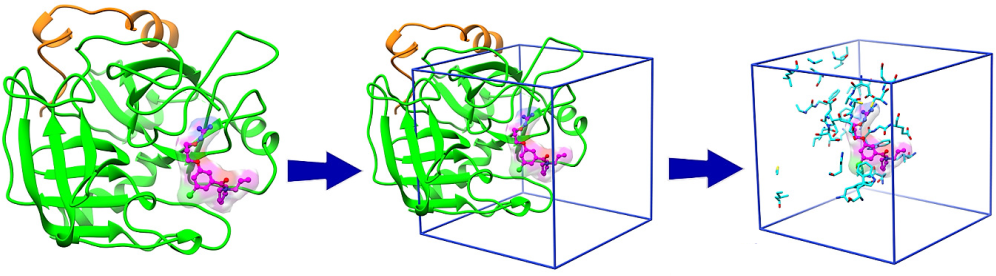
\includegraphics[width=0.8\linewidth]{images/grid_top}
    \end{figure}
    \textbf{A 3D grid of dimensions $32\times32\times32$ \r{A}$^3$ with resolution 1
    \r{A} is created, centered on the ligand.}
    \vspace{2mm}
    \begin{enumerate}
        \item The greatest end-to-end distance of a ligand in PDBbind v.2016 is $\sim32$ \r{A}.
        \item The vdW radius of the heavy atoms found in PDBbind ligands is
        $\geq 1.4$ \r{A}.
    \end{enumerate}
\end{frame}


\begin{frame}{i. Rasterization (2/2)}
    \textbf{PCMax algorithm: when converting atoms to voxels, atoms-as-voxels
    have a continuous effect on their neighbors.}
    \vspace{3mm}

    For each voxel, its occupancy taken as the maximum of
    \begin{equation*}
        n(r_i) = 1 - \exp\left(-\left(\frac{r_{vdW, i}}{r_i}\right)^{12}\right)
    \end{equation*}
    over all atoms $i$, where $r_{vdW, i}$ is the $i^{th}$ atom radius and $r_i$ is the inter-voxel distance.
\end{frame}


\subsection{ii. Channelization}
\begin{frame}{ii. Channelization}
    \begin{columns}[c]
        \column{.4\textwidth}
        \textbf{The input to the network is}
        $\pmb{32\times32\times32\alert{\times24}}$: 12 channels each
        created from the ligand and protein.
        \begin{itemize}
            \item 1 excluded volume channel.
            \item 11 channels of atoms involved in 
            \href{http://biosig.unimelb.edu.au/arpeggioweb/calculate/}
            {certain interatomic interactions}.
        \end{itemize}
        \column{.6\textwidth}
        \begin{figure}
            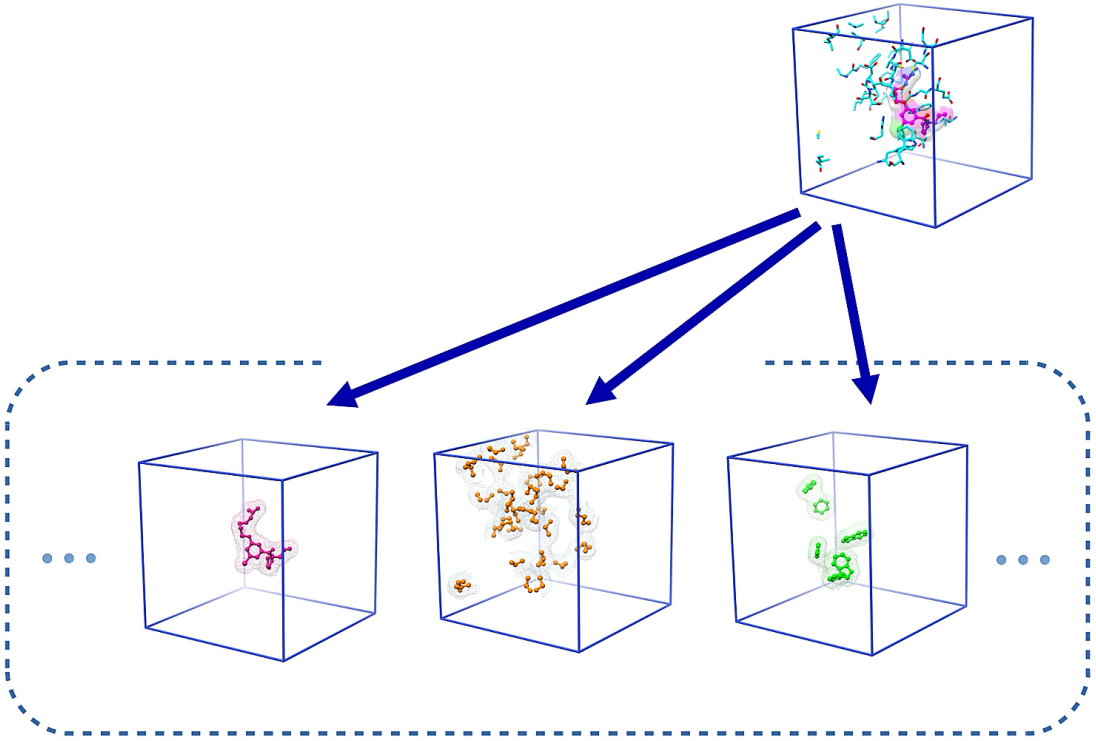
\includegraphics[width=\textwidth]{images/grid_bottom}
        \end{figure}
    \end{columns}
\end{frame}


%------------------------------------------------
\section{Network architecture}
%------------------------------------------------
\begin{frame}{The Three Block Overview}
    \begin{columns}[c]
        \column{.45\textwidth}
        \textbf{DeepAtom is relatively shallow, and has three blocks:}
        \begin{enumerate}
            \item Atom information integration block.
            \item Stacked feature extraction block.
            \item Global affinity regression block.
        \end{enumerate}
        \column{.6\textwidth}
        \begin{figure}
            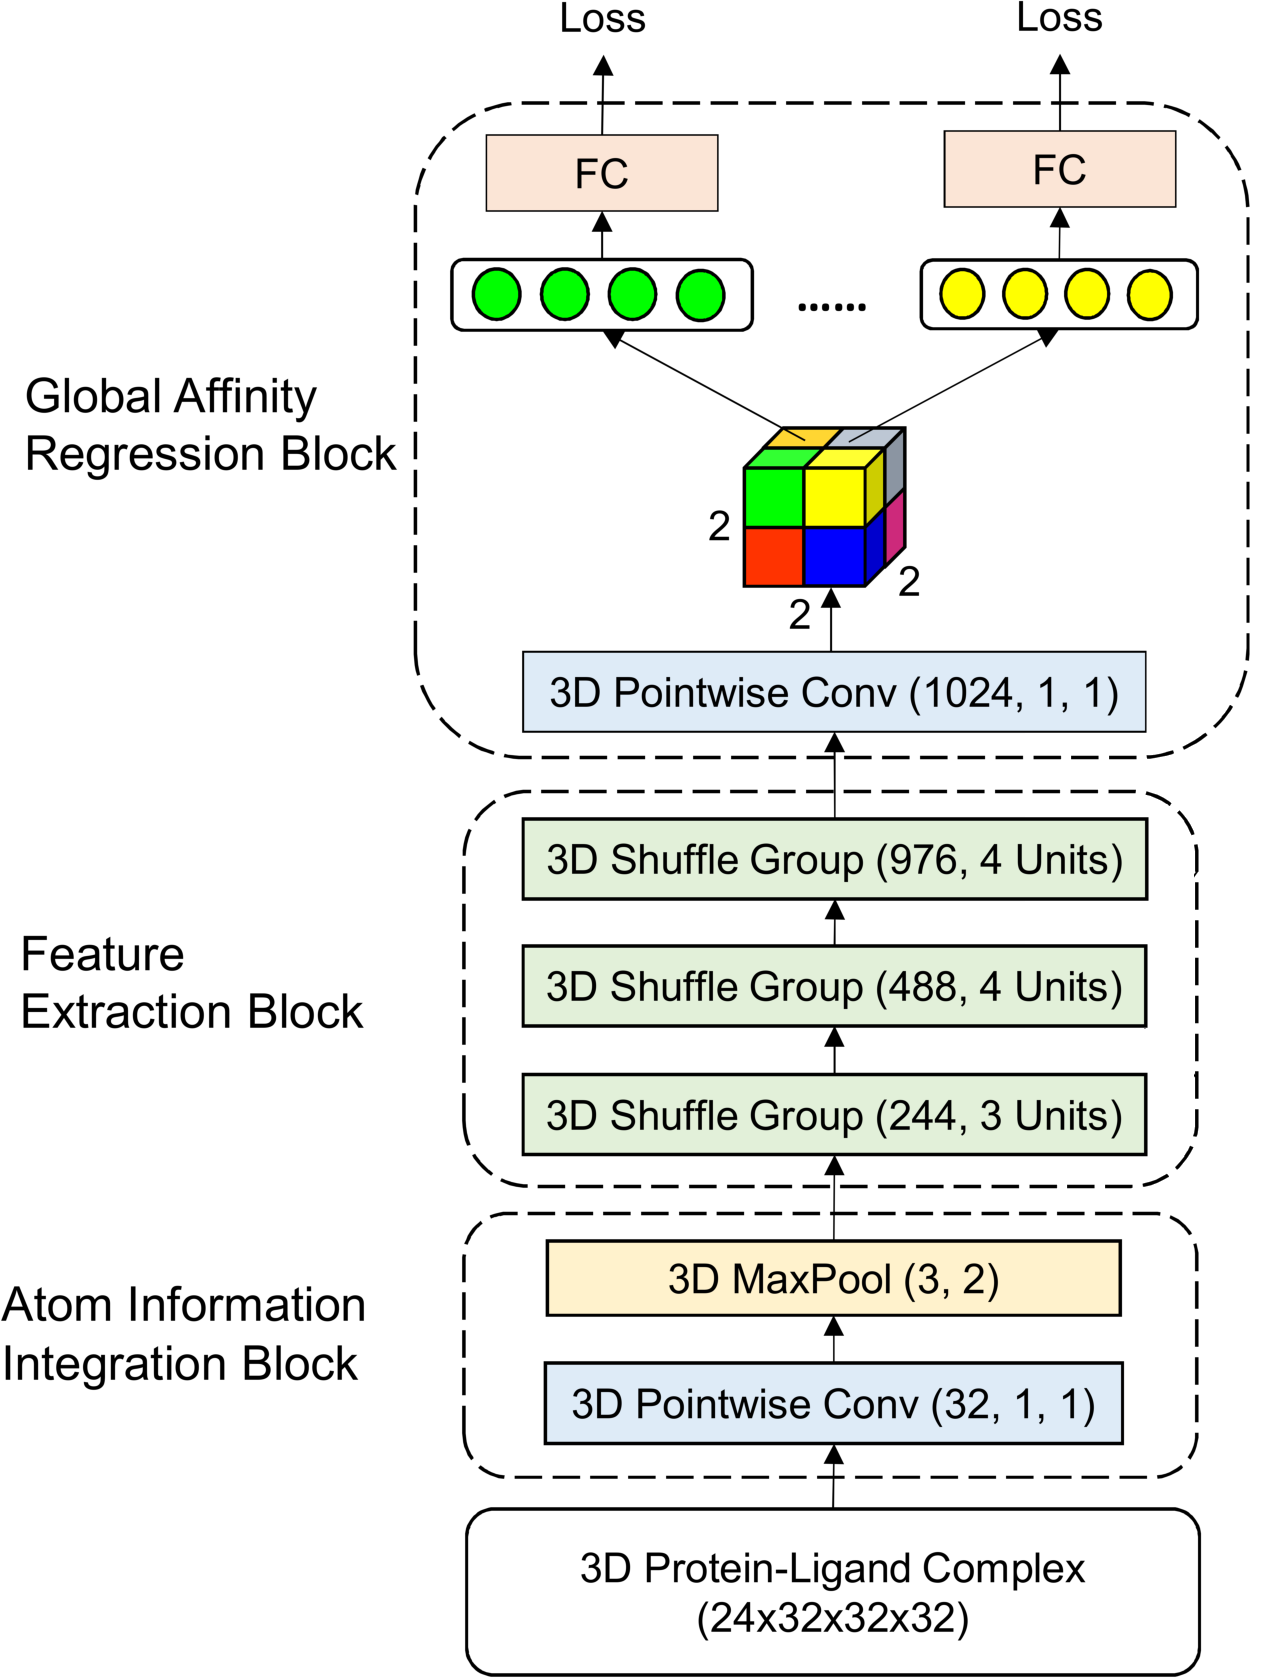
\includegraphics[width=0.55\textwidth]{images/network_left}
        \end{figure}
    \end{columns}
\end{frame}


\subsection{i. Atom information integration block}
\begin{frame}{i. Atom Information Integration Block}
    \textbf{Atomic information across the 24 channels is aggregate in a 
    pointwise fashion, and the output is then pooled.}
    \begin{enumerate}
        \item $\text{PWConv}(W, h)_{(i, j, k)} = \Sigma_{m}^{24}W_m\cdot 
        h_{(i,j,k,m)}$ is used to map the $24\times32^3$ input to $32^3$.
        \item The max-pooling downsamples the tensor to $16^3$.
    \end{enumerate}
    Semantically, this block processes the input into non-linear function of 
    the linear combination of the various channels (interaction types), 
    parsimoniously.
    \begin{figure}
        \centering
        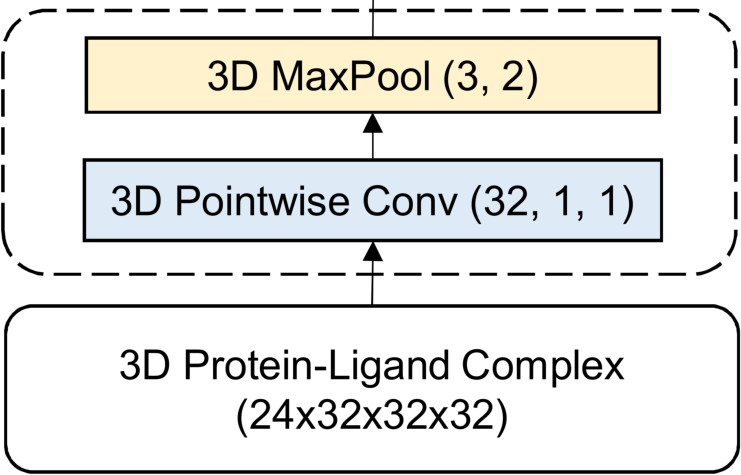
\includegraphics[width=0.3\textwidth]{images/aii_block}
    \end{figure}
\end{frame}


\subsection{ii. Stacked feature extraction block}
\begin{frame}{ii. Stacked Feature Extraction Block}
    \begin{columns}[c]
        \column{.45\textwidth}
        \textbf{Three 3D shuffle groups are stacked, each containing a parsimonious
        combination of pointwise and depthwise convolutions.}
        
        Shuffling, splitting, and then processing only certain channels encourages parsimonious while maintaining performance.
        \newline
        \begin{equation*}
            \text{DWConv}(W, h)_{(i, j, k)} =
        \end{equation*}
        \begin{equation*}
            \Sigma_{s,t,r}^{S, T, R} W_{s,t,r}\odot h_{(i+s,j+t,k+r)}
        \end{equation*}
        \column{.6\textwidth}
        \begin{figure}
            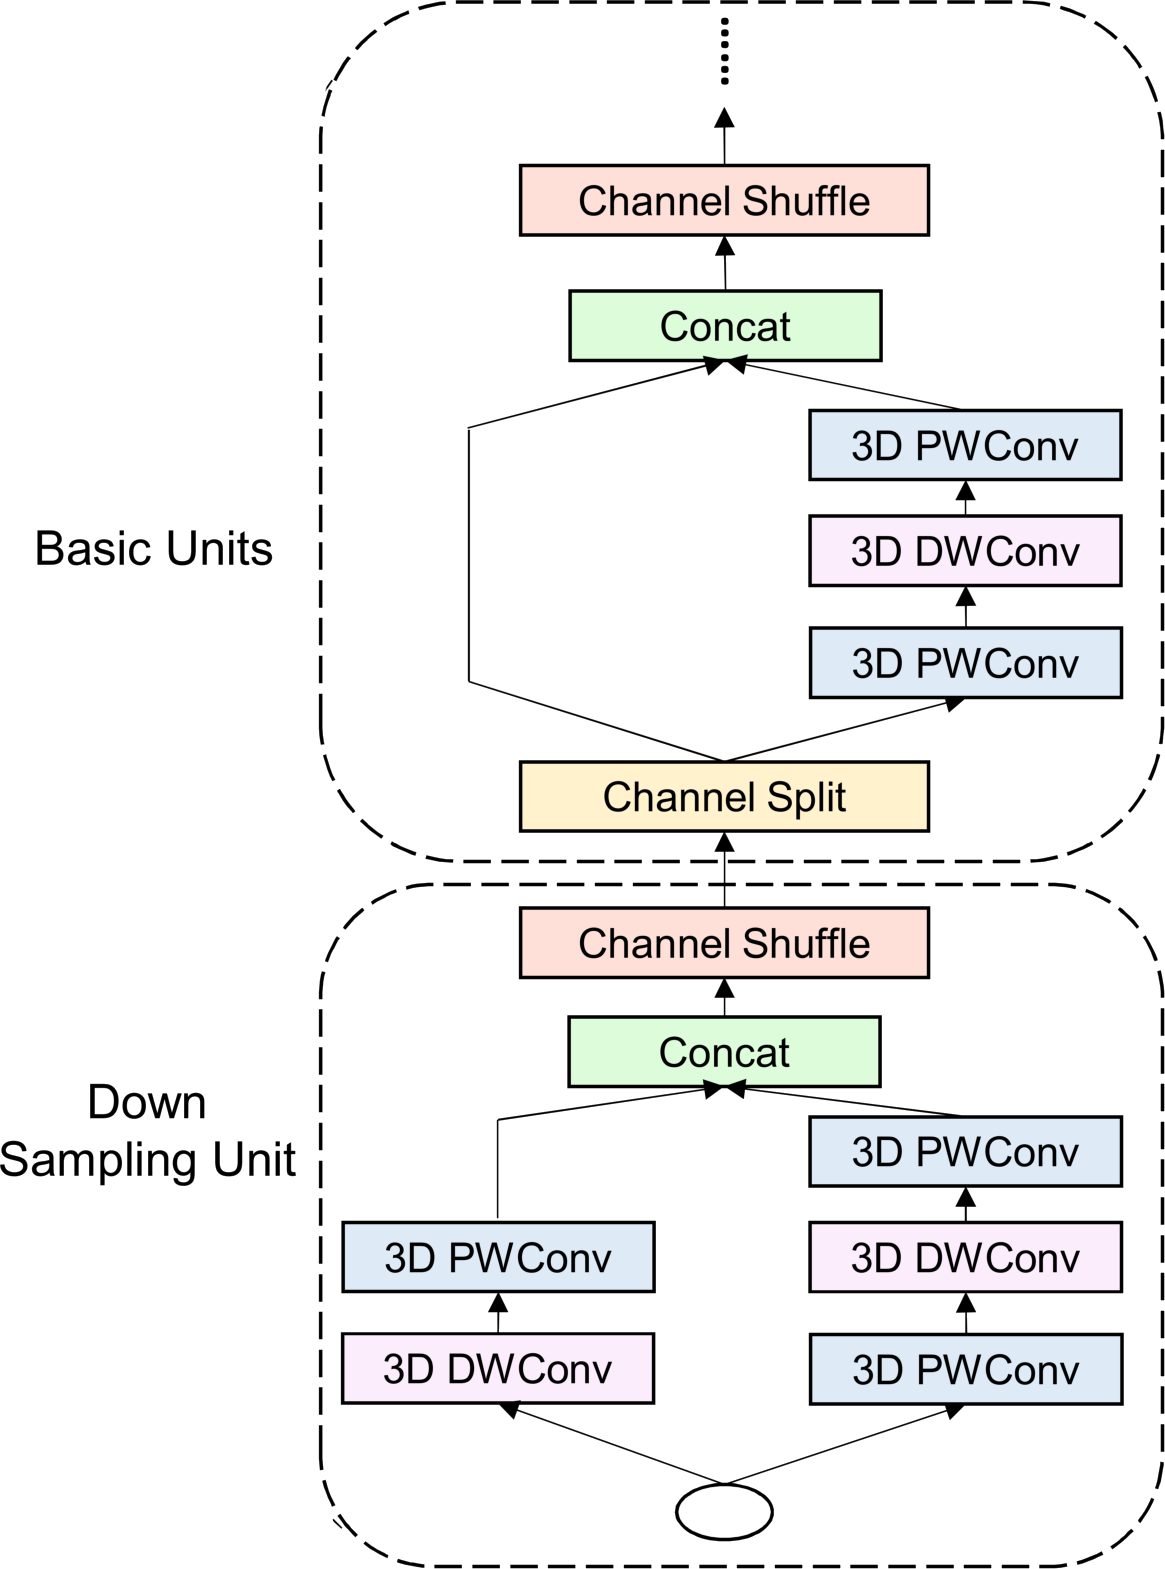
\includegraphics[width=0.55\textwidth]{images/network_right}
        \end{figure}
    \end{columns}
\end{frame}


\subsection{iii. Global affinity regression block}
\begin{frame}{iii. Global Affinity Regression Block}
    \begin{columns}[c]
        \column{.45\textwidth}
        \textbf{The output from the shuffle groups is downsampled and flattened into eight 
        1024-vectors.}
        \begin{itemize}
            \item Each vector represents the output from a distinct channel subset, and is 
            processed to create a BAP.
            \item The eight losses are used to train the network concurrently. During 
            evaluation, the eight vectors are averaged before a single BAP is created.
        \end{itemize}
        \column{.6\textwidth}
        \begin{figure}
            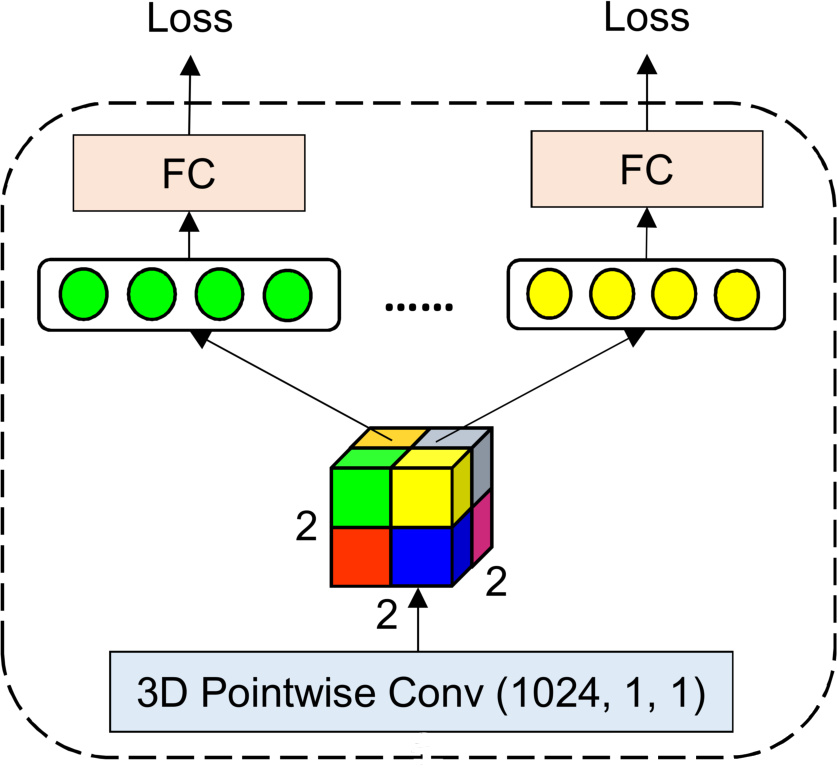
\includegraphics[width=0.7\textwidth]{images/gar_block}
        \end{figure}
    \end{columns}
\end{frame}


%------------------------------------------------
\section{Current progress}
%------------------------------------------------
\begin{frame}{Current Progress}
    \begin{enumerate}
        \item \textcolor{darkgreen}{Rasterize protein PDBs joined to ligand MOL2 files.}
        \begin{itemize}
            \item Done using Python's \texttt{HTMD} package.
        \end{itemize}
        \item \textcolor{darkgreen}{Channelize 3D grids.}
        \begin{itemize}
            \item Done using an offline implementation of Arpeggio's web service.
        \end{itemize}
        \item \textcolor{orange}{Implement DeepAtom architecture.}
        \begin{itemize}
            \item Shuffle groups expected to be a particular challenge.
        \end{itemize}
        \item \textcolor{darkred}{Train, tune, and validate DeepAtom on NSCC.}
        \begin{itemize}
            \item I have more ``low-level'' control over this DeepAtom implementation than
            I do of those of DrugVQA and GGNN.
        \end{itemize}
    \end{enumerate}
\end{frame}


%------------------------------------------------
\section{}
\begin{frame}{For More Details...}
    \footnotesize{
    DeepAtom:
    \begin{thebibliography}{99}
        \bibitem[Li et al., 2012]{p1} Li, Y., Rezaei, M. A., Li, C., \& Li, X. (2019)
        \newblock DeepAtom: A framework FOR Protein-Ligand binding affinity prediction
        \newblock \emph{IEEE/ACM Transactions on Computational Biology and Bioinformatics}.
    \end{thebibliography}
    \vspace{3mm}
    PCMax algorithm/rasterization of atoms:
    \begin{thebibliography}{99}
        \bibitem[Jiménez et al., 2017]{p1} Jiménez, J., Doerr, S., Martínez-Rosell, G., Rose, A. S., \& De Fabritiis, G. (2017)
        \newblock Deepsite: Protein-binding site predictor using 3d-convolutional neural networks
        \newblock \emph{Bioinformatics} 33(19), 3036-3042.
    \end{thebibliography}
    }
\end{frame}


\begin{frame}{For More Details...}
    \footnotesize{
    Arpeggio interatomic interaction finder:
    \begin{thebibliography}{99}
        \bibitem[Jubb et al., 2017]{p1} Jubb, H., Higueruelo, A., Ochoa-Montaño, B., Pitt, W., Ascher, D., \& Blundell, T. (2017)
        \newblock Arpeggio: A web server for calculating and visualising interatomic interactions in protein structures
        \newblock \emph{Journal of Molecular Biology} 429(3), 365-371.
    \end{thebibliography}
    \vspace{3mm}
    ShuffleNet:
    \begin{thebibliography}{99}
        \bibitem[Zhang et al., 2018]{p1} Zhang, X., Zhou, X., Lin, M., \& Sun, J. (2018)
        \newblock Shufflenet: An extremely efficient convolutional neural network for mobile devices
        \newblock \emph{2018 IEEE/CVF Conference on Computer Vision and Pattern Recognition}.
    \end{thebibliography}
    }
\end{frame}

\end{document}